\documentclass[11pt]{article}
\usepackage{tikz}
\usepackage{graphicx}
\usepackage[margin=1.0in]{geometry}
\usepackage{etoolbox}
\usepackage{amsmath}

\newcommand{\lessonheader}[2]{%
\begin{center} \Large {MA103: Data-Driven Modeling\\Lesson #1: #2}  \end{center}
\hrule
}

\newcommand{\objectiveitem}[1]{\item #1}
\newcommand{\lessonobjectives}[1]{%
\vspace{-0.1in}
\section*{Lesson Objectives}
\vspace{-0.1in}
\begin{enumerate}
\forcsvlist{\objectiveitem}{#1}
\end{enumerate}
\hrule
}

\newcommand{\subheader}[1]{%
\vspace{-0.1in}
\noindent
\section*{#1}
\vspace{-0.1in}
}

\newcommand{\subsubheader}[1]{%
\vspace{-0.1in}
\noindent
\subsubsection*{#1}
\vspace{-0.1in}
}

\begin{document}
\lessonheader{16}{Select, Use, Assess}

\lessonobjectives{%
  {Select an appropriate predictive model based on data, context, and purpose.},
  {Assess predictive models using training and test data.},
  {Interpret model outputs and limitations in context.},
  {Justify model selection and use for a given predictive modeling question.}%
}

\subheader{Warm-Up: Review of Non-Linear Functions}

What are the three types of non-linear functions we discussed during the previous class? What are their general forms?

\begin{table}[h]
    \centering
    \begin{tabular}{|p{0.3335\textwidth}|p{0.3335\textwidth}|}
        \hline
        \textbf{Function} & \textbf{General Form} \\
        \hline
        Linear & $y = ax + b$ \\
        \hline
         & \\
        \hline
         & \\
        \hline
         & \\
        \hline
    \end{tabular}
\end{table}

\noindent How do the parameters of each function change its shape?

\vfill

\noindent Is a polynomial a linear function? Is a linear function a polynomial?

\vfill

\begin{figure}[htbp] % [htbp] specifies placement preference (here, top, bottom, page)
    \centering % Centers the image horizontally
    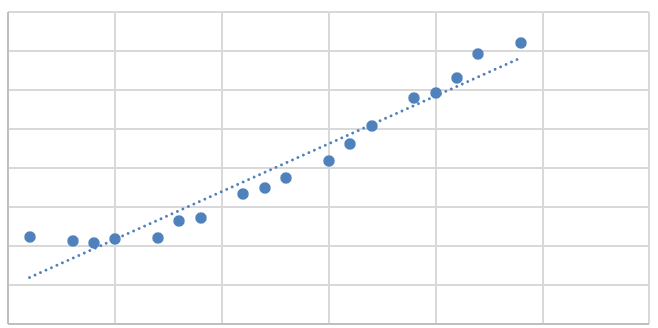
\includegraphics[width=0.6\textwidth]{Figures/1.png}
\end{figure}

\noindent How does the data shown in the image violate the assumptions of a linear model?

\vfill
\newpage

\hrule

\subheader{Exercise: Defend your Model}

As we proceed through the exercise, record observations and tools that are relevant to each phase of the modeling process. Consider how the ideas of \textit{selecting}, \textit{using}, and \textit{assessing} a model fit into the modeling framework we use in this class.
\begin{itemize}
\item FORMULATE

\vfill

\item SOLVE

\vfill

\item INTERPRET

\vfill

\item TEST

\vfill

\end{itemize}

\hrule


\subheader{Wrap-Up: Food for Thought}

\noindent Which model is the best? Does the answer depend on the situation the decision-maker is in?

\vfill

\noindent Is modeling a linear process, or is it circular/iterative? Is this true for both linear and non-linear modeling?

\vfill

\noindent Are there models (or tools for assessing models) that we did not cover in class, but that might have helped our decision maker? For two bonus points, bring in a short (3-5 handwritten sentences) discussion of one model or tool not covered in class that we could have applied to today's exercise. Due Monday, prior to the Predictive Modeling Gate.

\end{document}